\documentclass[12pt,letter]{article}
\usepackage[moduleName={Name Corp Octal Wave Generator}]{KautenjaDSP}
\begin{document}
\titlePage{img/Logo}{img/Module}{img/KautenjaDSP}

% -------------------
% MARK: Overview
% -------------------

\section{Overview}

Name Corp Octal Wave Generator is an emulation of the Namco 163 audio processing unit from the Nintendo Entertainment System (NES). The Namco 163 chip contains eight wave-table oscillators and 128 bytes of operational RAM for wave-table data. The wave-tables are 4-bit and can be as long as 63 samples. This module uses a bank of five 32-sample wave-tables to act as the waveform for all eight oscillators. Name Corp Octal Wave Generator provides the key features of the Namco 163 chip, namely,
\begin{itemize}
  \item \textbf{Octal waveform generator:} Eight wavetable oscillators with 18-bit frequency value
  \item \textbf{Waveform Morph:} Wavetable with 5 discrete 4-bit waveforms with length of $N = 32$ samples that can be interpolated between smoothly
  \item \textbf{4-bit Amplifier:} A 4-bit amplifier controls the output level of each oscillator with base/attenuator knobs and CV inputs
  \item \textbf{Namco 163 compute limitation:} activating each additional oscillator (up to 8) reduces the amount of compute available for all oscillators. This causes all oscillators to drop in frequency when additional oscillators are activated.
  \item \textbf{Channel Mixer:} Mix the voices together internally with hard clipping and intentional aliasing
\end{itemize}

% -------------------
% MARK: Panel Layout
% -------------------

\clearpage
\section{Panel Layout}

\begin{figure}[!htp]
\centering
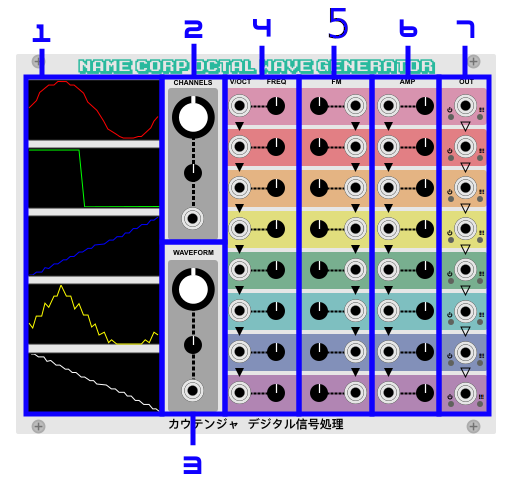
\includegraphics[width=\maxwidth{\textwidth}]{img/Interface}
\end{figure}

\subsection{Wavetable}

Each of the five waveforms in the table display on screens ordered from 1 to 5, top to bottom. Waveforms can be directly programmed into the module by clicking and dragging on a screen.

\subsection{Channels}

Individual voices on the module can be enabled to produce polyphonic effects. Due to computational limitations on the Namco 163 chip, the frequency range of each waveform generator drops when additional channels are enabled. The knob controls the number of active voices. Fully counter-clockwise enables only Voice 8 (in the bottom slot) with the highest frequency range. As the knob moves clockwise, additional voices are enabled and the frequency range of each voice is divided by a factor of $15$. The port provides an offset control from the knob's bias position where $1V$ increments correspond to a single voice level.

\subsection{Waveform}

The knob chooses between the five waveforms in the wavetable. Transitions between neighboring waveforms are smoothed using linear interpolation. When an input is patched to the port, the CV controls the offset from the trimpot's position. The position of the knob is offset by the CV in increments of $2V$.

\subsection{Frequency}

The trimpot controls the coarse frequency of the eight waveform generators. Frequency is quantized to an 18-bit value for the oscillators, which is particularly noticeable in the very low / high registers. The ports provide an exponential $V$/Octave input for controlling the pitch of the waveform generators. Inputs are reverse normalled forward from input 1 through to input 8.

\subsection{Frequency Modulation}

When nothing is patched to the frequency modulation port, the trimpot can be used to fine tune the frequency of the given waveform generator. When a signal is patched, the input port provides linear frequency modulation to the corresponding waveform generator and the trimpot can be used as an attenuverter to attenuate / polarize the incoming signal. Inputs are normalled forward from input 1 through to input 8.

\subsection{Amplifier}

When no input is connected, the trimpot controls the given waveform generator volume level with 4-bit resolution (i.e., $\in [0, 15]$). When an input is patched to the port, the trimpot acts like an attenuator that scales the CV control over the volume level. Because the amplifier has 4-bit control, the envelope of the voice will sound quantized when used with an external envelope generator. Inputs are normalled forward from input 1 through to input 8.

\subsection{Outputs}

Each voice produces an output signal of at most $10V_{pp}$ when the amplifier is maxed out. The individual oscillators cannot be overdriven to produce clipping, distortion, or aliasing. However, outputs are normalled forward into a sum mix where hard clipping \textit{can} occur. Excess clipping will introduce an aliasing effect to the mix. Outputs in the mix are clipped \textit{before} being normalled to the next output. VU meter lights, indicated by 
\includegraphics[height=\baselineskip]{img/VU}, measure the output of individual channels going from off ($-\infty dB$ to $-12dB$), to green ($-12dB$ to $0dB$), and lastly to red ($0dB$ to $3dB$) when clipping begins to occur. Channel power lights, indicated by 
\includegraphics[height=\baselineskip]{img/OnOff}, show whether the given channel is enabled according to the channel knob and CV.

% -------------------
% MARK: Data Sheet
% -------------------

\clearpage
\section{Data Sheet}

\begin{table}[!htp]
\begin{tabular}{|l|l|}
\hline
Type             & Oscillator               \\
\hline
Size             & 32 HP Eurorack           \\
\hline
Depth            & NA                       \\
\hline
Power            & NA                       \\ % 2 x 5 Eurorack
\hline
$+12V$ draw (mA) & 0 mA                     \\
\hline
$-12V$ draw (mA) & 0 mA                     \\
\hline
$+5V$ draw (mA)  & 0 mA                     \\
\hline
Sample Rate      & Programmable             \\
\hline
Bit Depth        & 16-bit                   \\
\hline
\end{tabular}
\end{table}

% -------------------
% MARK: References
% -------------------

\clearpage
\renewcommand\refname{References}
\nocite{*}
\bibliographystyle{apalike}
\bibliography{references}

\end{document}
